\documentclass[12pt]{article}
\usepackage[brazil]{babel}
\usepackage[utf8]{inputenc}
\usepackage{amsmath}
\usepackage{natbib}
\usepackage{listings}
\usepackage{color}

\definecolor{codegreen}{rgb}{0,0.6,0}
\definecolor{codegray}{rgb}{0.5,0.5,0.5}
\definecolor{codepurple}{rgb}{0.58,0,0.82}
\definecolor{backcolour}{rgb}{0.95,0.95,0.92}

\lstdefinestyle{mystyle}{
  backgroundcolor=\color{backcolour},
  commentstyle=\color{codegreen},
  keywordstyle=\color{red},
  numberstyle=\tiny\color{codegray},
  stringstyle=\color{codepurple},
  basicstyle=\footnotesize,
  breakatwhitespace=false,
  breaklines=true,
  captionpos=b,
  keepspaces=true,
  numbers=left,
  numbersep=5pt,
  showspaces=false,
  showstringspaces=false,
  showtabs=false,
  tabsize=2
}

\lstset{style=mystyle}
\usepackage{url}
\usepackage{amsmath}
\usepackage{float}
\usepackage{graphicx}
\graphicspath{{images/}}
\usepackage{parskip}
\usepackage{fancyhdr}
\usepackage{vmargin}
\setmarginsrb{3 cm}{2.5 cm}{3 cm}{2.5 cm}{1 cm}{1.5 cm}{1 cm}{1.5 cm}

\title{Zeros de Funções }								% Title
\author{Wilton Rodrigues}								% Author
\date{\today}											% Date

\makeatletter
\let\thetitle\@title
\let\theauthor\@author
\let\thedate\@date
\makeatother

\pagestyle{fancy}
\fancyhf{}
\lhead{\centering{\thetitle}}
\cfoot{\thepage}

\begin{document}

%%%%%%%%%%%%%%%%%%%%%%%%%%%%%%%%%%%%%%%%%%%%%%%%%%%%%%%%%%%%%%%%%%%%%%%%%%%%%%%%%%%%%%%%%

\begin{titlepage}
  \centering
  \begin{figure}[H]
    \centering
    
\includegraphics[width=0.7\textwidth]{logo.png}\\[2.0 cm]
  \end{figure}
  \textsc{\LARGE Universidade de Brasília}\\[2.5 cm]	% University Name
  \textsc{\Large Relatório de atividade do módulo 1}\\[0.5 cm]				% Activity name
  \textsc{\large Métodos Numéricos para Engenharia}\\[1.5 cm]				% Course Name
  \rule{\linewidth}{0.2 mm} \\[0.4 cm]
  {\huge \bfseries \thetitle}\\
  \rule{\linewidth}{0.2 mm} \\[2.5 cm]

  \begin{minipage}{0.4\textwidth}
    \begin{flushleft} \large
      \emph{Aluno:}\\
      \theauthor
    \end{flushleft}
  \end{minipage}
  \begin{minipage}{0.4\textwidth}
    \begin{flushright} \large
      \emph{Matrícula:} \\
      13/0049212									% Your Student Number
    \end{flushright}
  \end{minipage}\\
  \vspace*{0.5in}
  {\large \thedate}\\[0.5 cm]

  \vfill

\end{titlepage}

%%%%%%%%%%%%%%%%%%%%%%%%%%%%%%%%%%%%%%%%%%%%%%%%%%%%%%%%%%%%%%%%%%%%%%%%%%%%%%%%%%%%%%%%%
\tableofcontents
\pagebreak
%%%%%%%%%%%%%%%%%%%%%%%%%%%%%%%%%%%%%%%%%%%%%%%%%%%%%%%%%%%%%%%%%%%%%%%%%%%%%%%%%%%%%%%%%

\section{Introdução}

O objetivo deste relatório é exercitar os conceitos aprendidos em aula, com relação ao tópico: Zeros de funções. Que tem como objetivo prover métodos matemáticos capazes de determinar o ponto, ou pontos, nos quais a equação cruza ou toca o eixo X, ou seja, um valor numérico que satisfaça à equação. Tarefa que pode dispender um enorme esforço, ou em alguns casos é até mesmo impossível, em equações que não possuem solução analítica. Como é o caso da Equação de Kepler que é dada por:
\begin{equation} \label{eq:original}
  M = x - E sin(x)
\end{equation}
Dado que $E = 0.2$ e $M = 0.5$, o objetivo deste trabalho é obter a raíz da equação~\eqref{eq:original} com precisão de 10 casas decimais.

Fazendo as devidas substituições e manipulações matemáticas, obtemos a seguinte equação:
\begin{eqnarray}\label{eq:inzero}
  -E sin(x) + x - M = 0 \nonumber\\
  -0.2sin(x) + x - 0.5 = 0
\end{eqnarray}

A partir da equação~\eqref{eq:inzero}, utilizaremos dois passos para encontrar a raíz: O passo 1 tem como objetivo obter um intervalo $[a,b]$ aproximado no qual $x \in [a,b]$. O passo 2 é onde aplicaremos o método numérico da Bissecção para refinar a solução.

\section{Metodologia}

Neste primeiro passo, será feita uma análise da equação, baseando-se no gráfico da mesma e nos conceitos teóricos e teoremas do método escolhido. O sucesso ou falha do próximo passo está diretamente ligado aos resultados obtidos nesta fase de análise.
Baseando-se no teorema:
\newtheorem{ambiente}{Teorema}
\begin{ambiente}[Função Contínua]\label{teo:teorema}
Seja f(x) uma função contínua num intervalo [a,b]. Se f(a)f(b) $<$ 0, então existe pelo menos um ponto
x = $\alpha$ entre a e b que é zero de f(x).
\end{ambiente}

E analisando o gráfico da figura \ref{fig:grafico} é possível perceber que a equação~\eqref{eq:inzero} intercepta o eixo X no intervalo $[0,1]$

Ao substituirmos estes pontos na equação~\eqref{eq:inzero}, obtemos os seguintes resultados.

\begin{eqnarray}\label{eq:results}
  a = 0, b = 1 \nonumber\\
  f(a) =   -0.2sin(0) + 0 - 0.5 \nonumber\\
  f(a)= -0.5\nonumber\\
  f(b) =   -0.2sin(1) + 1 - 0.5 \nonumber\\
  f(b)= 0.3317058030384207 \nonumber\\
  f(a) * f(b) = -0.16585290151921034
\end{eqnarray}

Então, de acordo com o teorema \ref{teo:teorema}, como o resultado de $f(a) * f(b) < 0$ de fato há uma raíz entre o intervalo $[0,1]$.

\begin{figure}[!h]
  \centering
  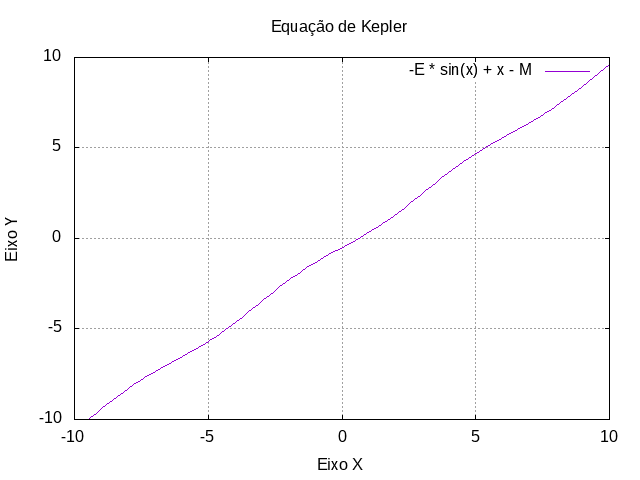
\includegraphics[width=15cm]{kepler.png}\\
  \caption{Plotagem da função no intervalo $[-10,10]$}\label{fig:grafico}
\end{figure}

\newpage
\section{Diagrama esquemático de execução}

Nesta seção, encontra-se o fluxo de execução da solução da equação~\eqref{eq:original} utilizando a linguagem C. Que é apresentada na próxima sessão.

\begin{figure}[!h]
  \centering
  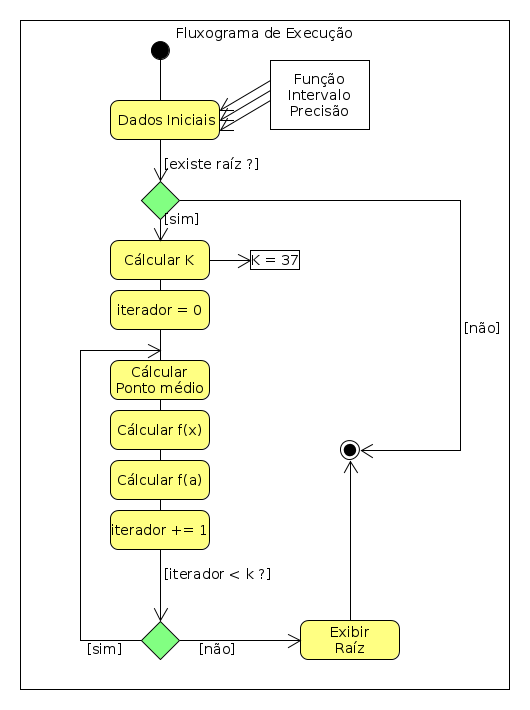
\includegraphics[width=10cm]{fluxograma.png}\\
  \caption{Fluxo de execução da solução}\label{fig:fluxo}
\end{figure}

A solução elaborada neste relatório funciona da seguinte maneira. Tanto a função, quanto a precisão desejada são inseridas diretamente no código fonte. Apenas o intervalo no qual se deseja verificar a existencia da raíz é solicitado ao usuário em tempo de execução. Caso o intervalo informado não possua uma raíz, de acordo com teorema \ref{teo:teorema}, uma mensagem é apresentada ao usuário e a execução encerra. Caso o intervalo seja válido a raíz correspondente é apresentada e então o programa se encerra.

\newpage
\section{Código Fonte}

\lstinputlisting[language=C]{../solution/m1.c}

\newpage
\section{Resultados e discussões}

%%%%%%%%%%%%%%%%%%%%%%%%%%%%%%%%%%%%%%%%%%%%%%%%%%%%%%%%%%%%%%%%%%%%%%%%%%%%%%%%%%%%%%%%%

\end{document}
